\documentclass[conference]{IEEEtran}
\IEEEoverridecommandlockouts

\usepackage{iftex}
\ifXeTeX
  \usepackage{fontspec}
  \setmainfont{texgyretermes}[Extension=.otf, UprightFont=*-regular, BoldFont=*-bold, ItalicFont=*-italic, BoldItalicFont=*-bolditalic]
  \setsansfont{texgyreheros}[Extension=.otf, UprightFont=*-regular, BoldFont=*-bold, ItalicFont=*-italic, BoldItalicFont=*-bolditalic]
\fi
\usepackage{cite}
\usepackage{amsmath,amssymb}
\usepackage{graphicx}
\usepackage{booktabs}
\usepackage{array}
\usepackage{tabularx}
\usepackage{url}
\usepackage{xcolor}
\usepackage{tikz}
\usetikzlibrary{positioning,arrows.meta,shapes.geometric,fit,calc,backgrounds}
\usepackage[hidelinks]{hyperref}

\graphicspath{{figures/}}
\newcommand{\rs}{Rs.\,}
\newcommand{\code}[1]{\texttt{\small #1}}
\newcolumntype{L}[1]{>{\raggedright\arraybackslash}p{#1}}

\begin{document}

\title{EcoInsight: Grounding a Small Open-Weight LLM in Live Indian Market Data with Serverless Retrieval and a Provenance Policy}

\author{\IEEEauthorblockN{Shivam Sharma}
\IEEEauthorblockA{\textit{Manav Rachna International}\\
\textit{Institute of Research and Studies}\\
Faridabad, India\\
ss18244646@gmail.com}
\and
\IEEEauthorblockN{Gaurav Kumar Mehra}
\IEEEauthorblockA{\textit{Manav Rachna International}\\
\textit{Institute of Research and Studies}\\
Faridabad, India\\
gmehra161@gmail.com}
\and
\IEEEauthorblockN{Ansh Tripathi}
\IEEEauthorblockA{\textit{Manav Rachna International}\\
\textit{Institute of Research and Studies}\\
Faridabad, India\\
anshtripathi259@gmail.com}}

\maketitle

\begin{abstract}
General-purpose large language models (LLMs) answer financial questions from frozen training data, so they quote stale prices and produce precise-looking figures that are not real. We present EcoInsight, an India-focused economic intelligence assistant that grounds a 20-billion-parameter open-weight model (gpt-oss-20b) in market data fetched at query time. Its retrieval layer, Search-Sync, uses deterministic rules to decide when to retrieve, runs three fetchers in parallel (benchmark context, entity-resolved stock quotes, and web search), and injects the results into the system prompt as a labelled authority block. A six-category provenance policy lets the model issue forecasts and buy/hold/sell verdicts while reserving the label ``verified fact'' for figures that were actually retrieved. A single per-symbol quote cache keeps the chatbot and every dashboard on the same price, with a worst-case staleness of six minutes. In live runs on 15 October 2026, the assistant reported retrieved price, P/E, EPS, and 52-week figures exactly, the chat and dashboard surfaces agreed within the cache window, and answers separated retrieved facts from labelled assumptions, predictions, and recommendations. Measured design iterations cut index-loading latency from 5.9\,s to 2.2\,s and gave the two response modes distinct profiles (2.5\,s concise answers versus 63\,s analyst reports). We also propose an evaluation protocol for grounded financial assistants.
\end{abstract}

\begin{IEEEkeywords}
retrieval-augmented generation, large language models, financial question answering, hallucination, provenance, serverless systems
\end{IEEEkeywords}

%=====================================================================
\section{Introduction}
%=====================================================================

Retail investors increasingly ask chat assistants questions such as ``Is Reliance overvalued right now?''. A correct answer depends on figures that change by the minute: price, price-to-earnings (P/E) ratio, 52-week range, and index levels. An LLM answering from its weights either refuses or produces a fluent, wrong number. In finance, a confident wrong number does more harm than a refusal.

Retrieval-augmented generation (RAG) is the standard remedy~\cite{lewis2020rag}, but most RAG work assumes a static corpus and a vector index. Market data differs in three ways. It is structured. It expires within minutes. And the same figure appears on several surfaces of a product (a chatbot, a dashboard, a ticker) that must agree with each other.

EcoInsight is a working web application built for this setting. It pairs a streaming assistant (``Eko'') with live dashboards for Indian indices, equities, commodities, currencies, and institutional fund flows. We address three research questions:

\begin{itemize}
\item \textbf{RQ1.} Can a small open-weight model be grounded in live market data well enough to answer price and valuation questions using only serverless infrastructure and no vector store?
\item \textbf{RQ2.} How should a grounded assistant treat figures that were \emph{not} retrieved, so that it neither refuses to engage nor presents estimates as facts?
\item \textbf{RQ3.} Which caching and prompting choices keep figures consistent across surfaces and keep latency acceptable?
\end{itemize}

Our contributions are:
\begin{enumerate}
\item \emph{Search-Sync}, a query-time retrieval pipeline built from rule-based gating, three parallel fetchers, and a shared 3-minute quote cache (Section~\ref{sec:method}).
\item A \emph{six-category provenance policy} that separates verified facts from derived values, assumptions, predictions, interpretations, and recommendations (Section~\ref{sec:provenance}).
\item A \emph{cross-surface consistency design} that keeps chatbot and dashboard prices identical within a bounded staleness window (Section~\ref{sec:consistency}).
\item An \emph{empirical study} of the deployed system: measured design iterations drawn from 391 commits, and live runs against real market data (Section~\ref{sec:eval}).
\end{enumerate}

%=====================================================================
\section{Related Work}
%=====================================================================

\textbf{Retrieval augmentation.} Lewis et al.~\cite{lewis2020rag} condition generation on passages retrieved from a dense index. EcoInsight keeps the core idea but replaces the index with structured quote lookups and live web search, because its key facts expire within minutes. Vu et al.~\cite{vu2023freshllms} show that inserting fresh search-engine results into the prompt substantially improves answers to fast-changing questions. Search-Sync is a domain-specific instance of that approach.

\textbf{Tool use.} Toolformer~\cite{schick2023toolformer} trains a model to decide when to call external tools. EcoInsight takes the opposite route: deterministic rules decide which tools to call before the model runs. This is predictable and cheap, and it works with a model that was never fine-tuned for tool use.

\textbf{Financial LLMs.} BloombergGPT~\cite{wu2023bloomberggpt} trains a 50B-parameter model on financial text, and FinGPT~\cite{yang2023fingpt} argues for open, frequently refreshed financial models. Both store domain knowledge in the weights, which goes stale between training runs. FinanceBench~\cite{islam2023financebench} reports that GPT-4-Turbo with a retrieval system answered incorrectly or refused 81\% of its questions. That result motivates EcoInsight's emphasis on structured, query-time data and on explicit handling of figures that were not retrieved.

\textbf{Hallucination and evaluation.} Ji et al.~\cite{ji2023survey} survey hallucination in text generation. FActScore~\cite{min2023factscore} breaks long answers into atomic facts and checks each, and Ragas~\cite{es2023ragas} measures how faithful a RAG answer is to its retrieved context. EcoInsight's provenance policy asks the model to tag each of its own atomic facts by origin, which makes those tags checkable by such tools (Section~\ref{sec:protocol}).

%=====================================================================
\section{System Architecture}
%=====================================================================

EcoInsight has three tiers (Fig.~\ref{fig:arch}): a React single-page client, a set of Vercel serverless functions, and a Supabase PostgreSQL database. All market data and model traffic passes through the serverless tier, which holds every secret and owns the shared quote cache. The codebase has 104 tracked files and roughly 17{,}000 lines of JavaScript. Table~\ref{tab:components} lists the main components.

\begin{figure*}[t]
\centering
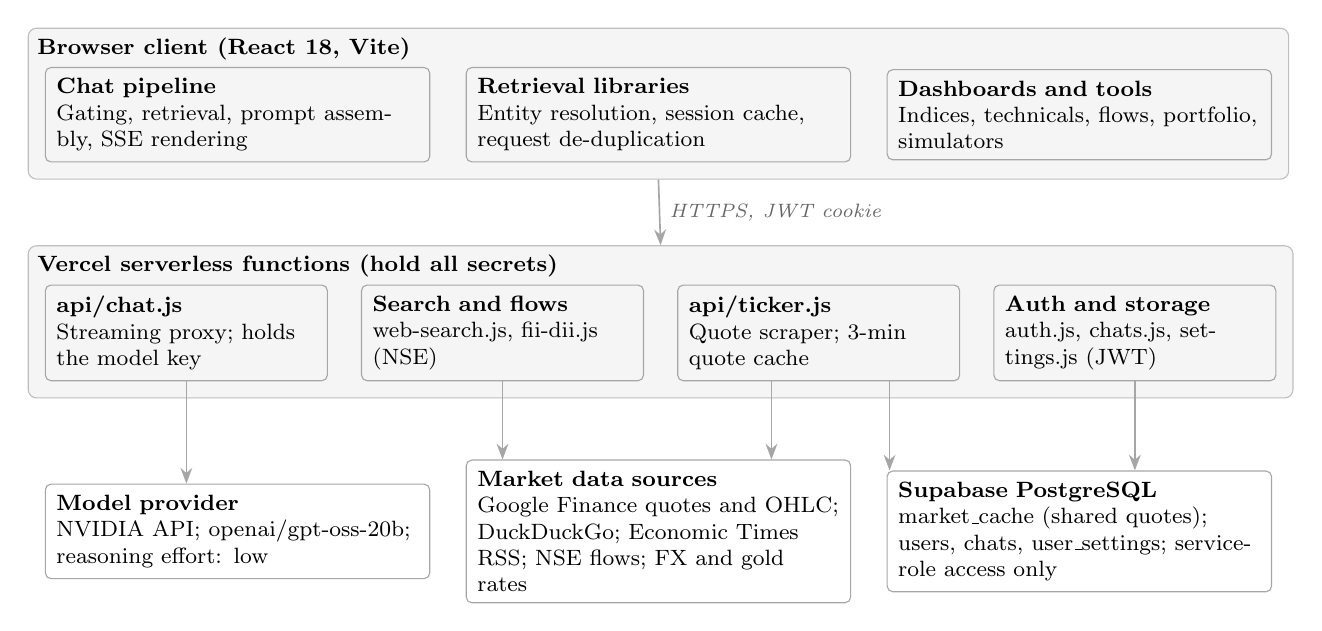
\begin{tikzpicture}[
  font=\footnotesize,
  box/.style={draw=gray!70, rounded corners=2pt, align=left, text width=#1, inner sep=4pt, minimum height=1.05cm},
  box/.default=3.6cm,
  tier/.style={draw=gray!50, fill=gray!8, rounded corners=3pt, inner sep=6pt},
  arr/.style={-{Stealth[length=2mm]}, gray!70, semithick},
  lbl/.style={font=\scriptsize\itshape, text=gray!80!black}
]
% client tier
\node[box=4.6cm] (c1) {\textbf{Chat pipeline}\\Gating, retrieval, prompt assembly, SSE rendering};
\node[box=4.6cm, right=0.45cm of c1] (c2) {\textbf{Retrieval libraries}\\Entity resolution, session cache, request de-duplication};
\node[box=4.6cm, right=0.45cm of c2] (c3) {\textbf{Dashboards and tools}\\Indices, technicals, flows, portfolio, simulators};
\begin{scope}[on background layer]
\node[tier, fit=(c1)(c3), inner ysep=10pt, yshift=4pt, label={[anchor=north west, font=\footnotesize\bfseries]north west:Browser client (React 18, Vite)}] (client) {};
\end{scope}
% server tier
\node[box=3.3cm, below=1.55cm of c1.south west, anchor=north west] (s1) {\textbf{api/chat.js}\\Streaming proxy; holds the model key};
\node[box=3.3cm, right=0.42cm of s1] (s2) {\textbf{Search and flows}\\web-search.js, fii-dii.js (NSE)};
\node[box=3.3cm, right=0.42cm of s2] (s3) {\textbf{api/ticker.js}\\Quote scraper; 3-min quote cache};
\node[box=3.3cm, right=0.42cm of s3] (s4) {\textbf{Auth and storage}\\auth.js, chats.js, settings.js (JWT)};
\begin{scope}[on background layer]
\node[tier, fit=(s1)(s4), inner ysep=10pt, yshift=4pt, label={[anchor=north west, font=\footnotesize\bfseries]north west:Vercel serverless functions (hold all secrets)}] (server) {};
\end{scope}
% external tier
\node[box=4.6cm, below=1.3cm of s1.south west, anchor=north west] (e1) {\textbf{Model provider}\\NVIDIA API; openai/gpt-oss-20b; reasoning effort: low};
\node[box=4.6cm, right=0.45cm of e1] (e2) {\textbf{Market data sources}\\Google Finance quotes and OHLC; DuckDuckGo; Economic Times RSS; NSE flows; FX and gold rates};
\node[box=4.6cm, right=0.45cm of e2] (e3) {\textbf{Supabase PostgreSQL}\\market\_cache (shared quotes); users, chats, user\_settings; service-role access only};
% arrows
\draw[arr] (client.south) -- node[right, lbl] {HTTPS, JWT cookie} (server.north);
\draw[arr] (s1.south) -- (s1.south |- e1.north);
\draw[arr] (s2.south) -- (s2.south |- e2.north);
\draw[arr] ([xshift=-0.6cm]s3.south) -- ([xshift=-0.6cm]s3.south |- e2.north);
\draw[arr] ([xshift=0.9cm]s3.south) -- ([xshift=0.9cm]s3.south |- e3.north);
\draw[arr] (s4.south) -- (s4.south |- e3.north);
\end{tikzpicture}
\caption{Architecture. The browser never contacts a data source, the model, or the user tables directly. \code{api/ticker.js} both scrapes quotes and writes the shared cache that the chatbot and every dashboard read.}
\label{fig:arch}
\end{figure*}

\begin{table}[t]
\caption{Main Components}
\label{tab:components}
\centering
\footnotesize
\begin{tabular}{@{}L{1.0cm}L{2.85cm}L{3.75cm}@{}}
\toprule
Tier & Component & Role \\
\midrule
Client & \code{App.jsx} & Global state, view routing, chat pipeline, PDF export \\
Client & 33 view components & Dashboards, simulators, 3D visuals (Recharts, Three.js) \\
Client & Retrieval libraries (3 files) & Entity resolution, context assembly, session cache \\
Server & \code{api/chat.js} & Streams provider responses; key stays server-side \\
Server & \code{api/ticker.js} & Quotes, fundamentals, $\sim$1 month of daily OHLC \\
Server & \code{api/web-search.js} & DuckDuckGo HTML results; Economic Times RSS fallback \\
Server & \code{api/fii-dii.js} & Provisional FII/DII cash-market flows from NSE \\
Server & \code{auth}, \code{chats}, \code{settings} & Accounts; storage scoped by verified JWT \\
Data & Supabase & \code{users}, \code{user\_settings}, \code{chats}, \code{market\_cache} \\
\bottomrule
\end{tabular}
\end{table}

\textbf{Model choice.} The assistant runs gpt-oss-20b~\cite{openai2025gptoss} through NVIDIA's hosted API with \code{reasoning\_effort} fixed at ``low''. With this reasoning model, hidden reasoning tokens share the output budget with the visible answer; ``low'' effort leaves that budget for the answer itself, and response depth is controlled by the prompt and the token ceiling instead. The server, not the client, selects the model, so a model change takes effect for every user at once.

\textbf{Authentication.} Users sign up with an email and password (bcrypt-hashed, minimum 8 characters) or through Google OAuth. The server issues a signed JWT in an HTTP-only, SameSite=Lax cookie that is valid for 30 days. Every storage endpoint verifies that cookie and scopes its queries to the token's user ID in code.

%=====================================================================
\section{Methodology}
\label{sec:method}
%=====================================================================

\subsection{Search-Sync: Query-Time Grounding}

Search-Sync (Fig.~\ref{fig:flow}) decides with fixed rules whether a query needs live data, fetches three kinds of context in parallel, and places the result in the system prompt under a labelled authority block. No model call is spent on retrieval decisions.

\begin{figure}[t]
\centering
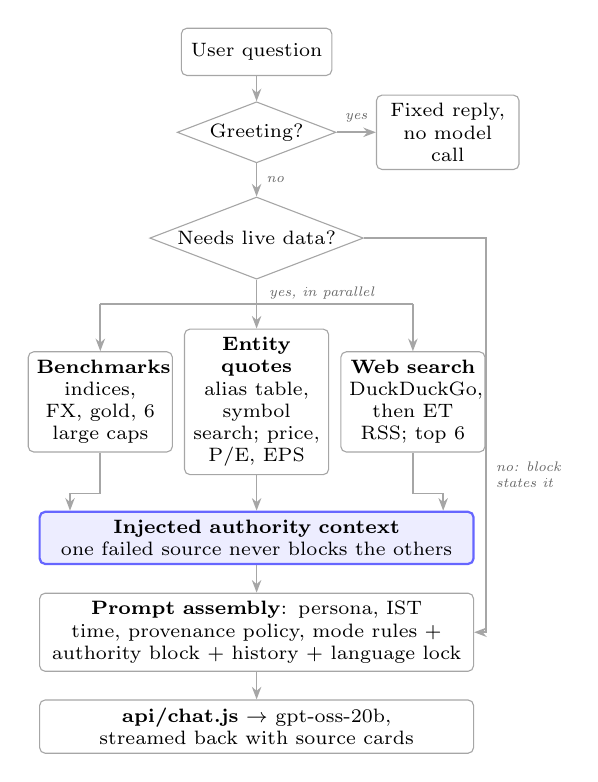
\begin{tikzpicture}[
  font=\scriptsize,
  node distance=0.42cm,
  step/.style={draw=gray!70, rounded corners=2pt, align=center, text width=#1, inner sep=3pt, minimum height=0.6cm},
  step/.default=2.3cm,
  dec/.style={draw=gray!70, diamond, aspect=2.6, align=center, inner sep=1pt},
  key/.style={draw=blue!60, fill=blue!7, thick, rounded corners=2pt, align=center, text width=5.3cm, inner sep=3pt},
  arr/.style={-{Stealth[length=1.6mm]}, gray!70, semithick},
  lbl/.style={font=\tiny\itshape, text=gray!80!black}
]
\node[step=1.7cm] (q) {User question};
\node[dec, below=0.32cm of q] (g) {Greeting?};
\node[step=1.6cm, right=0.5cm of g] (fx) {Fixed reply,\\no model call};
\node[dec, below=0.42cm of g] (n) {Needs live data?};
\node[step=1.62cm, below=0.62cm of n] (f2) {\textbf{Entity quotes}\\alias table, symbol search; price, P/E, EPS};
\node[step=1.62cm, left=0.14cm of f2] (f1) {\textbf{Benchmarks}\\indices, FX, gold, 6 large caps};
\node[step=1.62cm, right=0.14cm of f2] (f3) {\textbf{Web search}\\DuckDuckGo, then ET RSS; top 6};
\node[key, below=0.45cm of f2] (a) {\textbf{Injected authority context}\\one failed source never blocks the others};
\node[step=5.3cm, below=0.35cm of a] (p) {\textbf{Prompt assembly}: persona, IST time, provenance policy, mode rules + authority block + history + language lock};
\node[step=5.3cm, below=0.35cm of p] (m) {\textbf{api/chat.js} $\rightarrow$ gpt-oss-20b, streamed back with source cards};
\draw[arr] (q) -- (g);
\draw[arr] (g) -- node[above, lbl] {yes} (fx);
\draw[arr] (g) -- node[right, lbl] {no} (n);
\coordinate (bus) at ($(n.south)!0.5!(f2.north)$);
\draw[gray!70, semithick] (n.south) -- (bus);
\draw[gray!70, semithick] (f1.north |- bus) -- (f3.north |- bus);
\draw[arr] (f1.north |- bus) -- (f1.north);
\draw[arr] (bus) -- (f2.north);
\draw[arr] (f3.north |- bus) -- (f3.north);
\node[lbl, right=1pt of bus, yshift=4pt] {yes, in parallel};
\draw[arr] (f1.south) |- ($(a.north west)+(0.4,0.22)$) -- ++(0,-0.22);
\draw[arr] (f2.south) -- (a.north);
\draw[arr] (f3.south) |- ($(a.north east)+(-0.4,0.22)$) -- ++(0,-0.22);
\draw[arr] (a) -- (p);
\draw[arr] (p) -- (m);
\draw[arr] (n.east) -- ++(1.55,0) |- node[pos=0.3, right, lbl, align=left] {no: block\\states it} (p.east);
\end{tikzpicture}
\caption{Search-Sync request flow: two rule-based gates and three parallel fetchers. The model sees one labelled block whether retrieval succeeded, partly succeeded, or was not needed.}
\label{fig:flow}
\end{figure}

\emph{Gating.} A query is routed to retrieval when it contains one of 51 financial keywords (e.g., ``nifty'', ``p/e'', ``dividend'', ``rbi'') or has more than four words. Greetings in English and Hindi/Hinglish are answered from a fixed table without a model call. A 5-second client-side cooldown limits message rate.

\emph{Three fetchers.} Retrieval runs under \code{Promise.allSettled}, so one slow or failing source never blocks the others. (i)~\emph{Benchmark context}: Nifty~50, Sensex, and Nifty Bank levels; USD/INR, EUR/INR, and GBP/INR; Indian gold and silver rates; and cached quotes for six large caps with an advance/decline ratio. (ii)~\emph{Entity-resolved quotes}: company mentions are resolved in three passes. The first is a longest-match against a hand-built alias table (Nifty~50 names, about 60 mid caps, renamed listings such as Zomato$\rightarrow$ETERNAL, and seven US mega caps). The second sends capitalised phrases to Alpha Vantage symbol search, with results cached for 7 days. The third treats ALL-CAPS tokens as tickers. Up to five symbols are quoted with price, P/E, EPS, market capitalisation, 52-week and intraday range, dividend yield, and volume. (iii)~\emph{Web search}: the query is rewritten by appending ``India'' to financial questions that lack Indian context and the current year when no year is given. The server scrapes DuckDuckGo results and falls back to an Economic Times RSS feed. The client keeps up to six results that share a keyword with the question and shows them as source cards beneath the answer.

\emph{Quote resolution.} \code{api/ticker.js} maps aliases (indices, commodities, currencies, crypto) to Google Finance identifiers. A bare symbol is tried on NSE, then BSE, then NASDAQ, then as an NSE or BSE index, and finally on NYSE. Each page yields the quote, a fundamentals table, and about one month of daily OHLC bars. The scraper finds the bars by the shape of the embedded array, not by a fixed key, which keeps extraction stable when the page's internal keys are renumbered.

\emph{Prompt assembly.} The request contains: the system prompt (persona, current IST date and time, provenance policy, mode rules); an \code{INJECTED AUTHORITY CONTEXT} block holding everything retrieved; the chat history; the user message; and a language instruction (English, or mirror Hindi/Hinglish). When nothing was retrieved, the block states so explicitly and instructs the model to answer fully from its own knowledge, which keeps conceptual questions fully answered.

\subsection{One Price Everywhere}
\label{sec:consistency}

The chatbot, the Intelligence Hub dashboard, the news ticker, and the earnings panel all read prices through \code{api/ticker.js}. Consistency rests on three rules. First, the server caches the quote, fundamentals, and raw OHLC history under \emph{one key per symbol} with a 3-minute TTL. Chart series for each range (1D, 1W, 1M, 1Y) are derived fresh from that quote on every request instead of being cached separately, so every chart range shows the same headline price. Second, the dashboard's in-memory cache and the client-written grounding cache use the same 3-minute expiry, and forced refreshes are written back. Third, concurrent requests for one symbol share a single in-flight promise. Because two caches can stack, the worst-case age of a displayed price is
\begin{equation}
\Delta t_{\max} \approx \mathrm{TTL}_{\text{server}} + \mathrm{TTL}_{\text{client}} = 3 + 3 = 6~\text{min}.
\label{eq:staleness}
\end{equation}
The 1W and 1M charts (Fig.~\ref{fig:hub}) plot real daily closes taken from the quote page. The 1D and 1Y views are drawn as curves bounded by real values (today's open, high, and low; the 52-week high and low) that end at the live price.

\begin{figure}[t]
\centering
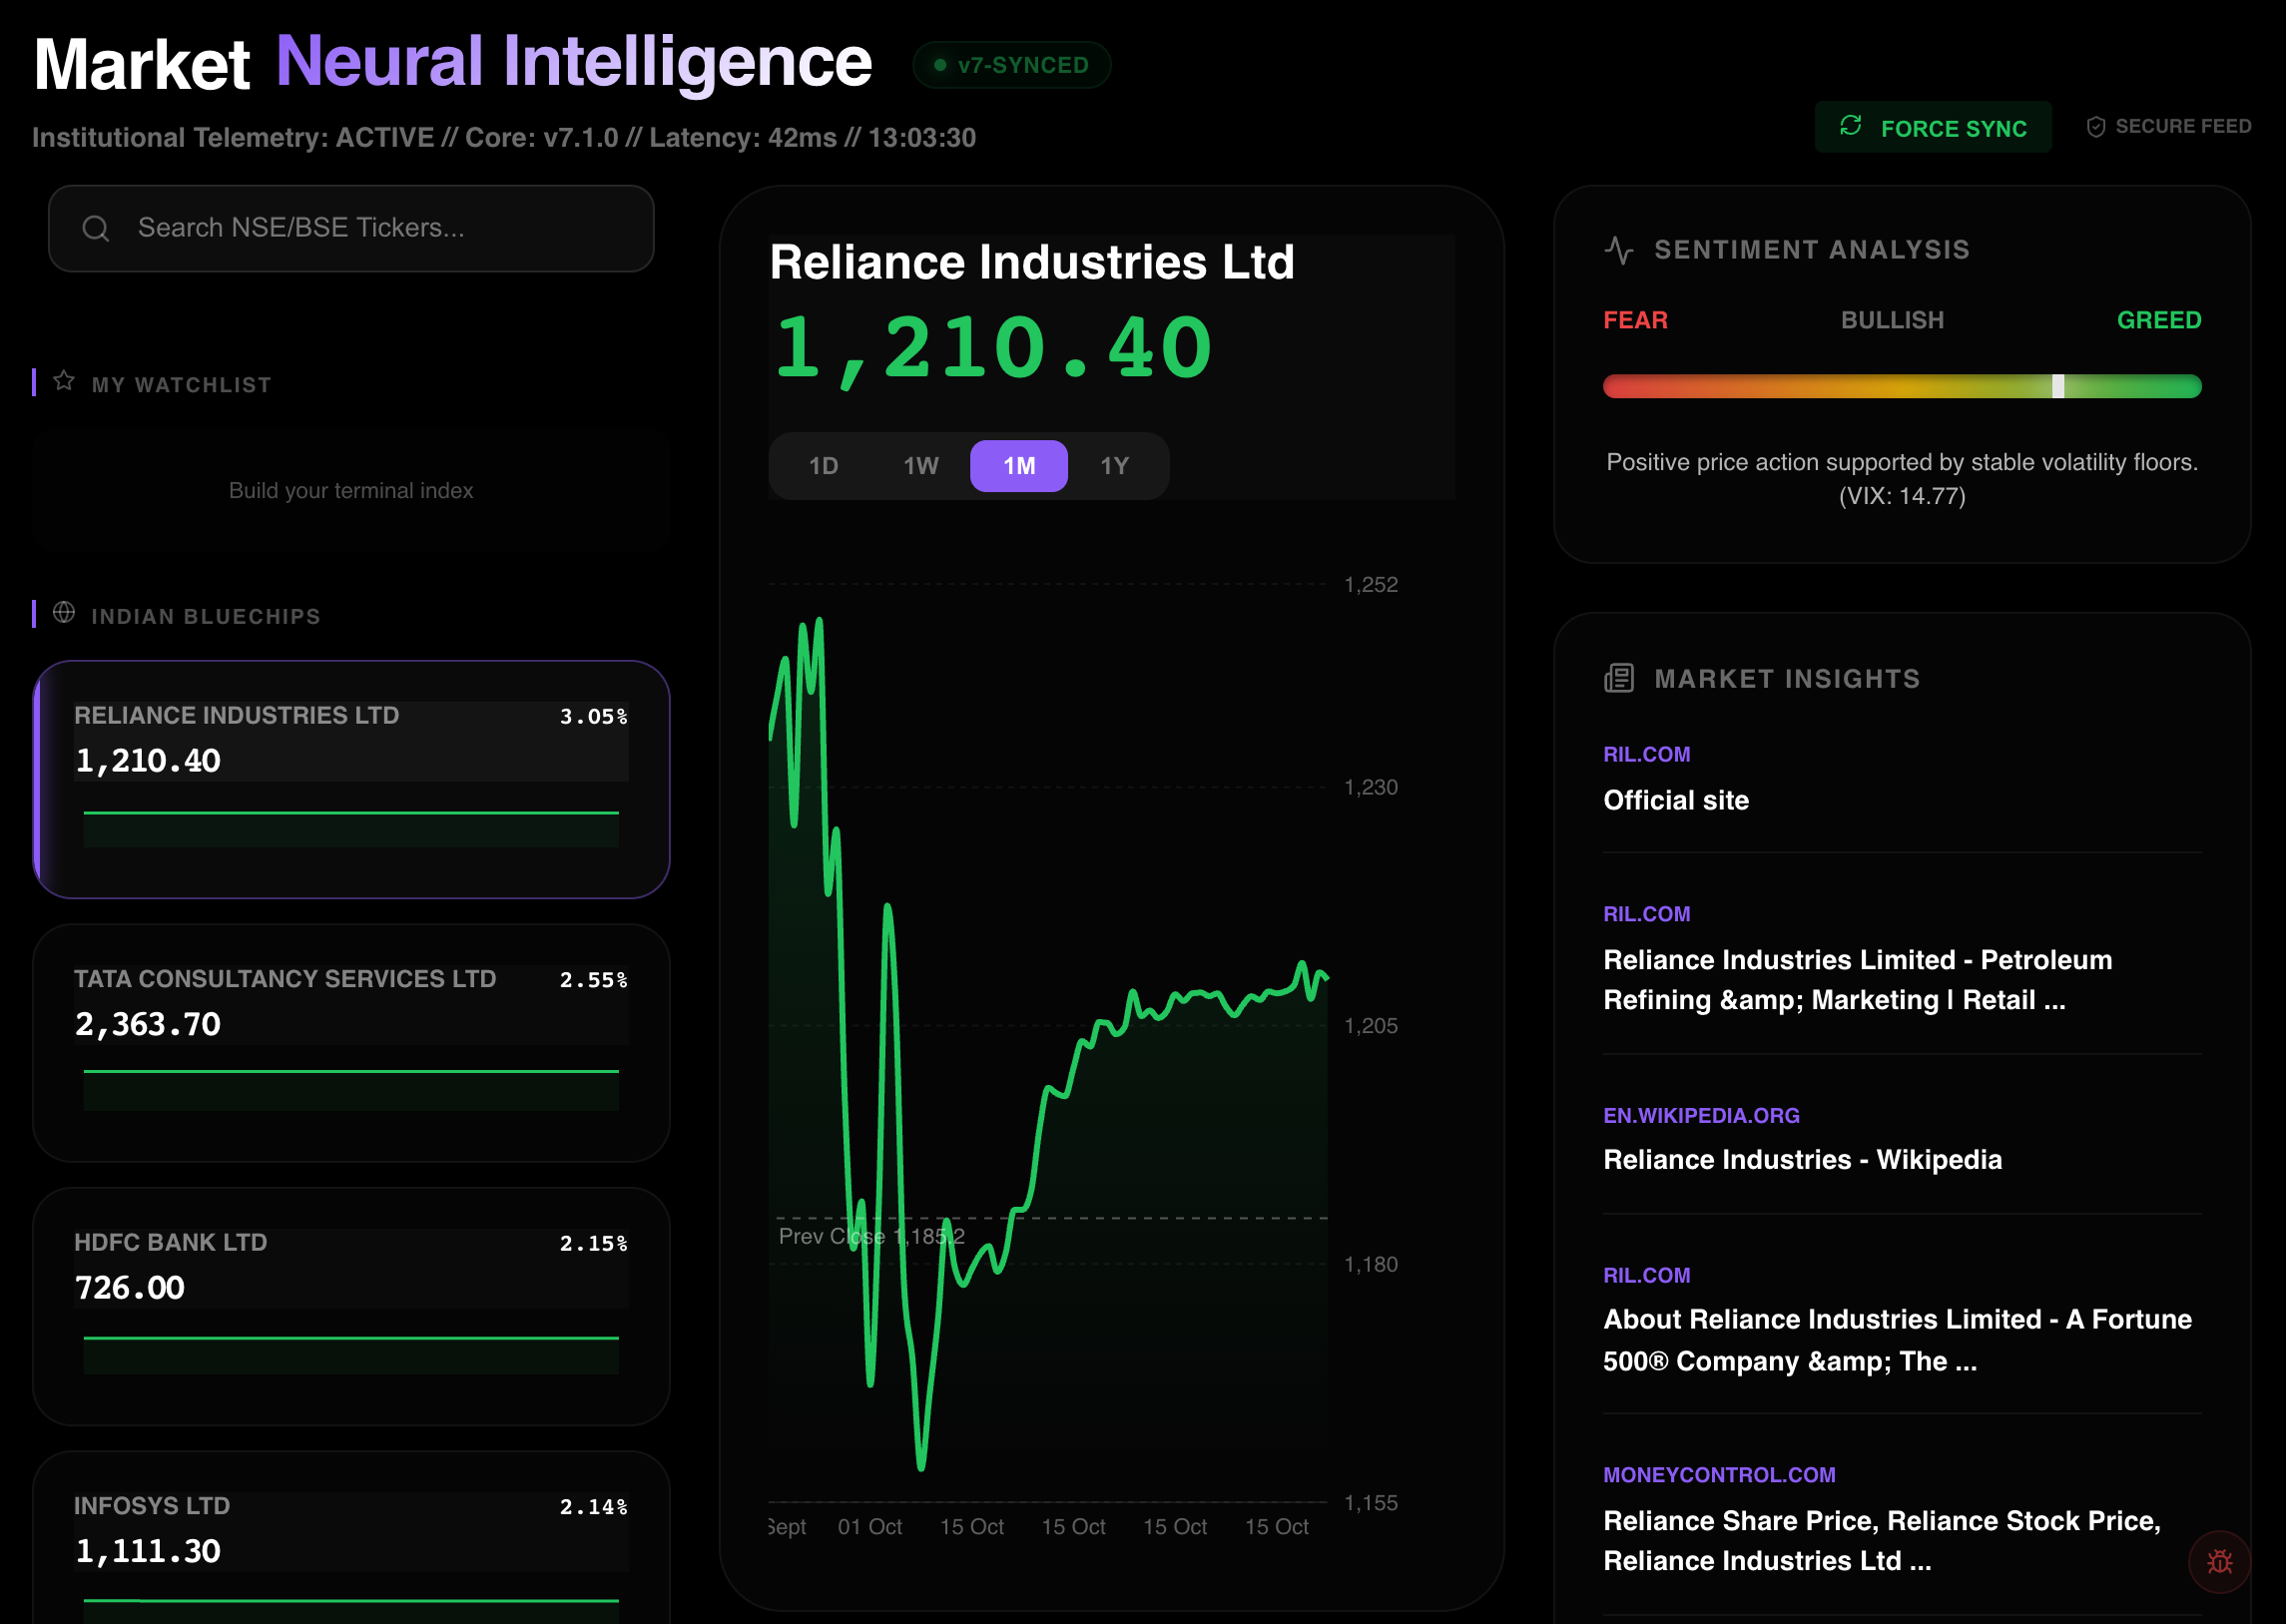
\includegraphics[width=\columnwidth]{fig-hub}
\caption{Eko Intelligence Hub, 1M range, 15 Oct 2026. The series is real daily closes. The dashed line marks the previous close. The headline price comes from the same quote cache the chatbot reads.}
\label{fig:hub}
\end{figure}

\subsection{Provenance Policy}
\label{sec:provenance}

The system prompt asks the model to assign every number to one of six categories (Table~\ref{tab:provenance}). The central rule is that the label ``verified fact'' is \emph{earned} only by figures present in the injected context. Three companion rules complete the policy. A \emph{no-refusal} rule requires the model to engage with every question from its own knowledge even when retrieval returns nothing. A \emph{no-fabrication} rule requires it to write ``not available in verified context'' for any missing current figure. \emph{Attribution} rules forbid citing analysts, filings, or URLs that are not in the context; inflating vague figures into false precision (``around 5\%'' into ``5.02\%''); and treating a missing value as zero. Every recommendation is presented as a labelled model output, not as regulated investment advice.

\begin{table}[t]
\caption{Six-Category Provenance Policy}
\label{tab:provenance}
\centering
\footnotesize
\begin{tabular}{@{}L{2.08cm}L{3.05cm}L{2.32cm}@{}}
\toprule
Category & Qualifies when & Example \\
\midrule
Verified fact & In injected context, or stable well-known knowledge & RBI target band 2--6\% \\
Derived value & Computed only from verified inputs; method stated & EPS = price / P/E \\
Assumption & An input the model chooses, stated as such & ``Assume 8\% growth'' \\
Prediction & Forward-looking estimate, labelled & ``Model target \rs1,450'' \\
Interpretation & Qualitative synthesis of the above & Valuation vs.\ growth \\
Recommendation & Verdict built on labelled factors & ``Verdict: Hold'' \\
\bottomrule
\end{tabular}
\end{table}

\subsection{Two Response Modes}

The two modes produce different kinds of answer, not just different lengths (Table~\ref{tab:modes}). Eco mode returns a short plain-text answer quickly. In High mode the model may also emit a fenced \code{chart} JSON block that the client renders with Recharts, and a \code{sentinel} block listing the sector effects of a scenario. Tagged blocks that do not parse are dropped rather than shown as raw JSON.

\begin{table}[t]
\caption{Response Modes (One Measured Query Each)}
\label{tab:modes}
\centering
\footnotesize
\begin{tabular}{@{}lL{2.3cm}L{2.0cm}L{1.6cm}@{}}
\toprule
Mode & Token budget & Format & Measured \\
\midrule
Eco & 500 (fixed) & 5--6 lines, plain text & 2.5\,s, 555 chars \\
High & 1{,}536 / 3{,}072 / 6{,}144 (Short / Medium / Long) & Tables, $\le$1 chart, $\le$1 scenario matrix & 63\,s, $\sim$6{,}000 chars \\
\bottomrule
\end{tabular}
\end{table}

%=====================================================================
\section{Implementation}
%=====================================================================

\subsection{Streaming and Resilience}
The chat proxy forwards the provider's server-sent event stream unchanged, so the API key stays on the server and the client keeps a standard streaming parser. The client retries twice, after 1\,s and 2\,s, on HTTP~429, any 5xx response, or a network error. It paces rendering at 20\,ms per chunk. In High mode an 8-second minimum ``analysis'' animation runs before the answer appears; Eco mode skips it.

\subsection{Derived Market Indicators}
Every dashboard indicator is a fixed formula over the same quotes the chatbot uses, not a model output. Breadth sentiment over the cached large-cap set is
\begin{equation}
S = \min\!\Big(100,\ \max\big(0,\ 50 + 10\,\overline{\Delta\%} + 5\,R_{AD}\big)\Big),
\label{eq:sentiment}
\end{equation}
where $\overline{\Delta\%}$ is the mean daily percentage change and $R_{AD}$ is the advance/decline ratio. A fear-and-greed gauge starts at 50, adds between $+20$ and $-30$ by India VIX band and between $+20$ and $-25$ by the Nifty~50 daily move, and is clamped to $[5, 95]$. Technicals (Wilder RSI-14, distance from the 20-day simple moving average, and the one-month move) are computed from Nifty~50's real daily closes. The economic calendar is generated from release rules: CPI on the 12th and WPI on the 14th (moved past weekends), quarterly GDP on the last weekday of February, May, August, and November, and RBI policy dates for FY~2026--27. Provisional FII/DII flows come from NSE and are cached for 30 minutes.

\subsection{Storage and Security Model}
All user data passes through serverless endpoints that verify the JWT cookie and use the Supabase service-role key, taking the user ID from the verified token. Anonymous and authenticated database roles have no grants on \code{users}, \code{chats}, or \code{user\_settings}, so the browser cannot query user tables directly. Only \code{market\_cache} is shared, and only the server writes to it.

%=====================================================================
\section{Evaluation}
\label{sec:eval}
%=====================================================================

We evaluate EcoInsight in two ways: design iterations whose effect was measured during development (Section~\ref{sec:devlog}), and live runs of the full stack against real market data (Section~\ref{sec:live}). Section~\ref{sec:protocol} proposes a benchmark protocol for comparing grounded financial assistants.

\subsection{Measured Design Iterations}
\label{sec:devlog}

The system was built over 391 commits between March and October 2026. Table~\ref{tab:devlog} lists the iterations that shaped grounding, consistency, latency, and security, with the effect measured at the time.

\begin{table*}[t]
\caption{Design Iterations and Their Measured Effect, 2026 (From Commit History)}
\label{tab:devlog}
\centering
\footnotesize
\begin{tabular}{@{}L{1.0cm}L{3.6cm}L{6.2cm}L{6.0cm}@{}}
\toprule
Date & Area & Change & Measured effect \\
\midrule
Oct 14 & Cross-surface consistency & Dashboard session cache given the same 3-min expiry as the server; forced refreshes written back; silent 3-min refresh & Chatbot and dashboard read one quote \\
Oct 14 & Live dashboard panels & FII/DII flows from NSE; calendar generated from release rules; RSI computed from real closes & Panels driven by live or rule-derived data \\
Sep 22 & Price freshness & One 3-min quote cache per symbol; chart series derived per request & Identical price on the 1D, 1W, and 1M views \\
Sep 15 & Provenance policy & Six categories; ``verified'' reserved for injected figures & Missing price reported as unavailable while a labelled target is still given \\
Sep 15 & Time-sensitive figures & Data-integrity rules for prices, rates, and inflation prints & Uncertain figures given as ranges with a pointer to RBI/MoSPI \\
Sep 15 & Coverage & Mandate scoped to injected figures; empty context stated explicitly & Conceptual questions answered fully \\
Sep 15 & Response modes & Separate prompt branches; fixed 500-token Eco budget & 2.5\,s Eco vs.\ 63\,s High answers \\
Sep 15 & Data isolation & User data moved behind server-side endpoints scoped by verified JWT; direct table grants revoked & Unauthenticated requests receive HTTP 401 \\
Sep 15 & Latency & Index quotes fetched in parallel; concurrent requests de-duplicated & 3 index lookups: 5.9\,s $\rightarrow$ 2.2\,s \\
Sep 15 & Structured output & Larger token budget; unparseable tagged blocks dropped & No raw JSON shown in chat \\
Sep 14 & Model serving & Server-side proxy; server selects gpt-oss-20b & API key kept server-only; 1--3\,s first response \\
\bottomrule
\end{tabular}
\end{table*}

Two patterns stand out. First, consistency is a property of the caching design rather than of the data source: unifying the quote cache per symbol is what made every surface and every chart range report the same price. Second, the provenance policy was refined iteratively, each version tested with and without injected data, until the model both engaged fully with every question and kept retrieved facts separate from its own estimates.

\subsection{Live System Runs}
\label{sec:live}

On 15 October 2026, between 13:00 and 13:20 IST during market hours, we ran the system (commit \code{497d294}) against the live model provider and live data sources. We asked the same Infosys valuation question twice in High mode, about ten minutes apart, and captured the Intelligence Hub at the same time.

\emph{Retrieved figures were reported exactly.} In both runs the assistant reported the injected price, P/E 15.01, EPS \rs74.02, and 52-week range \rs980.40--1,728.00, and attributed them to the retrieval engine (Fig.~\ref{fig:answer}a). The figures are internally consistent ($15.01 \times 74.02 = 1{,}111.0$, matching the reported price of \rs1,111).

\emph{Surfaces agreed.} The first run reported \rs1,111.60. The dashboards showed \rs1,111.30 at 13:02 and \rs1,111.45 at 13:03, so the chat and dashboard surfaces agreed to within 0.03\%, inside the refresh window of~(\ref{eq:staleness}).

\emph{Provenance labels were applied.} The first run placed its inputs under ``Model Assumptions'' with an explicit note that they were illustrative, its valuation under ``Model Prediction'', and its verdict under ``Recommendation''. The second run used ``Model Prediction / Forecast'' and ``Recommendation'' headings and gave verdicts per investor profile (Fig.~\ref{fig:answer}b). In both runs, forward-looking values were presented as estimates and never as retrieved facts.

\emph{Sources were shown.} Each answer ended with source cards for the retrieved web results (Economic Times, Livemint, Value Research, and others), so a reader can check the context the model was given.

\begin{figure}[t]
\centering
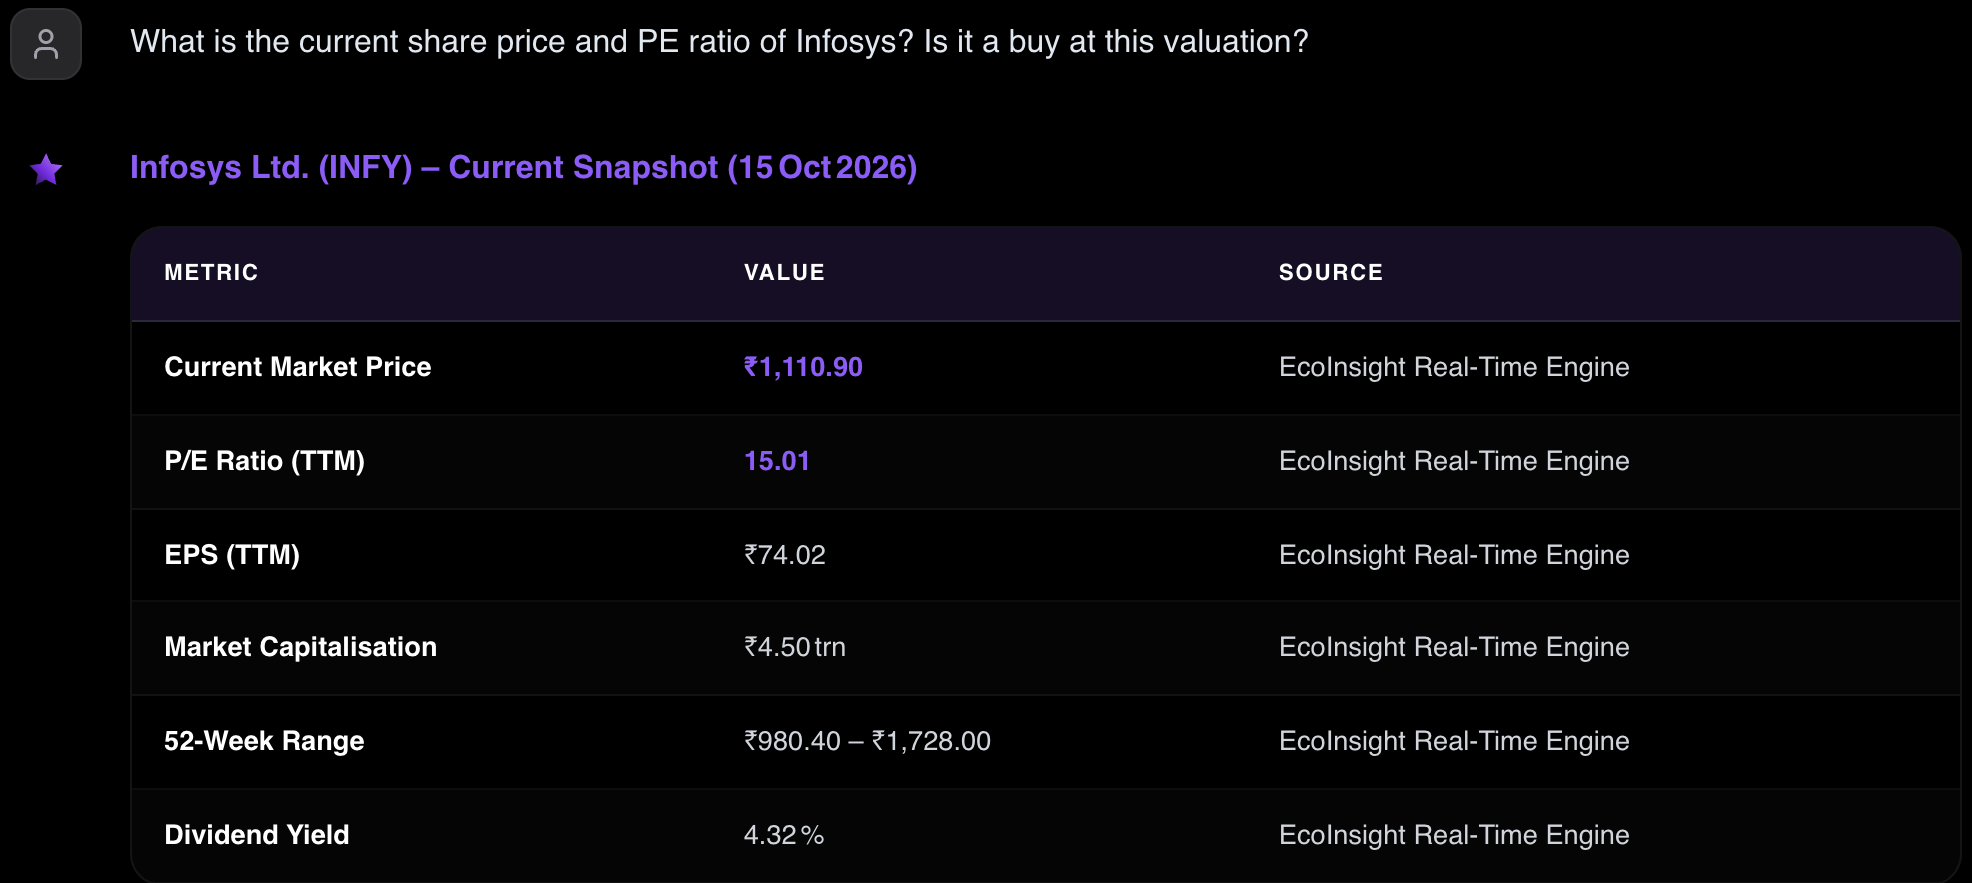
\includegraphics[width=\columnwidth]{fig-answer-table}\\[2pt]
{\footnotesize (a) Retrieved figures, reported verbatim with their source.}\\[6pt]
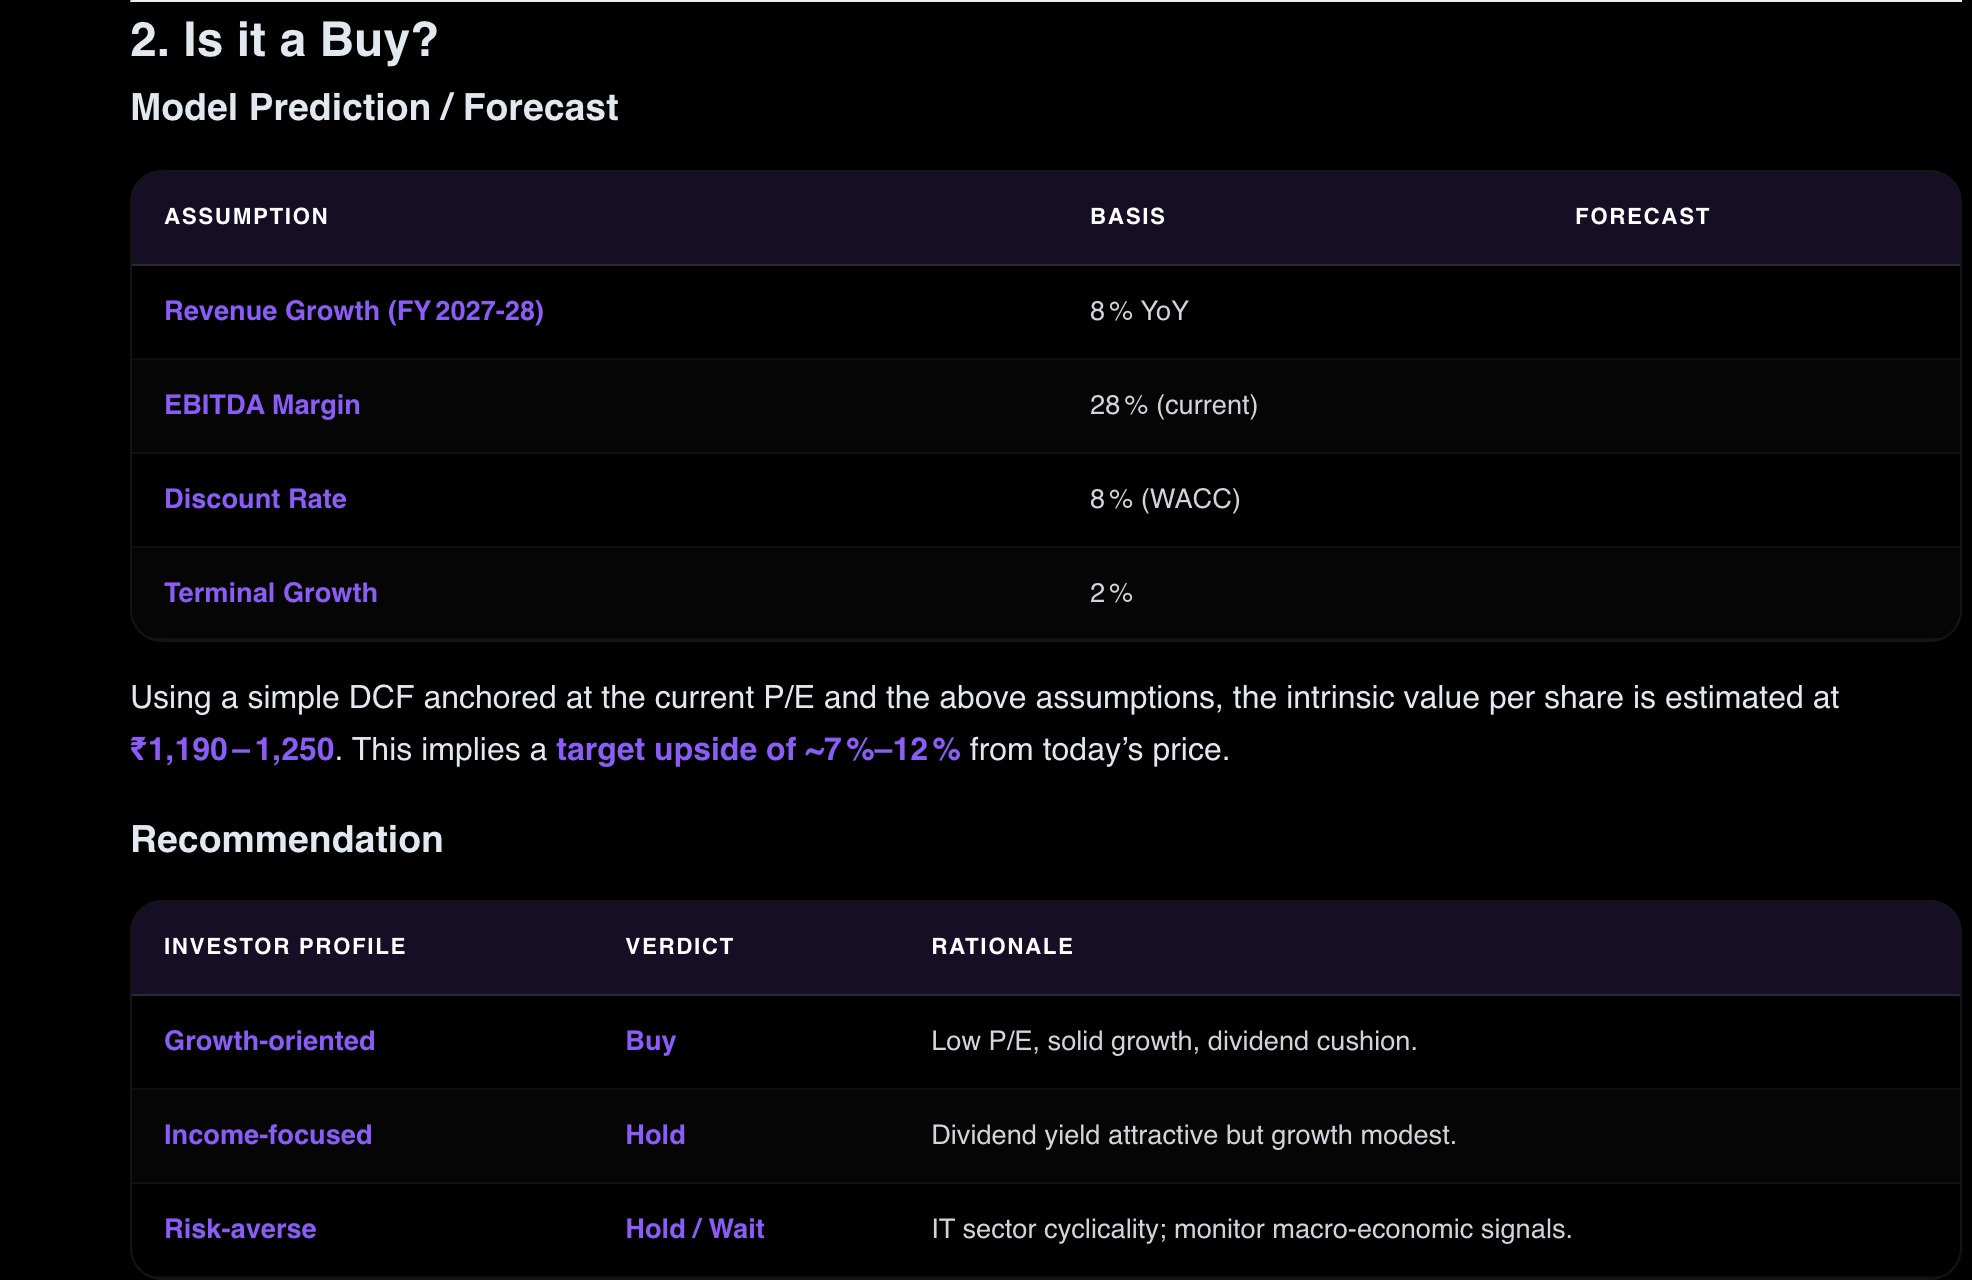
\includegraphics[width=\columnwidth]{fig-answer-forecast}\\[2pt]
{\footnotesize (b) Labelled forecast and per-profile verdicts.}
\caption{High-mode answer to ``What is the current share price and PE ratio of Infosys? Is it a buy at this valuation?'', 15 Oct 2026. Retrieved figures and the model's own estimates are kept under separate, labelled headings.}
\label{fig:answer}
\end{figure}

\subsection{Proposed Benchmark Protocol}
\label{sec:protocol}

To compare grounded financial assistants directly, we propose evaluating three configurations on a fixed question set: the model alone, retrieval without a provenance policy, and the full system. Questions should cover live price and valuation, macro statistics, conceptual explanation, and forecasting, each in English and Hindi/Hinglish. Each live question is paired with a reference quote captured when it is asked. Table~\ref{tab:protocol} defines the metrics.

\begin{table}[t]
\caption{Proposed Metrics}
\label{tab:protocol}
\centering
\footnotesize
\begin{tabular}{@{}L{1.85cm}L{5.6cm}@{}}
\toprule
Metric & Definition \\
\midrule
Numeric accuracy & Share of quoted figures within $\pm$0.5\% of the reference quote (tolerance covers~(\ref{eq:staleness})) \\
Fabrication rate & Share of specific figures in neither the context nor stable knowledge \\
Label precision & Share of ``verified'' figures that appear in the injected context \\
Derivation validity & Share of derived and predicted values reproducible from their stated inputs \\
Refusal rate & Share of answerable questions declined \\
Faithfulness & Ragas faithfulness to the retrieved context~\cite{es2023ragas} \\
Retrieval success & Share of gated queries where each fetcher returned data \\
Language fidelity & Share of answers in the language of the question \\
Latency & p50 and p95 time to first token and to completion, by mode \\
\bottomrule
\end{tabular}
\end{table}

%=====================================================================
\section{Conclusion and Future Work}
%=====================================================================

Live market grounding is practical without a vector store or a fine-tuned model. Rule-gated parallel retrieval, a shared 3-minute quote cache, and an explicit authority block let a 20B open-weight model report current Indian market figures exactly and consistently across surfaces (RQ1). The six-category provenance policy lets the assistant give forecasts and verdicts while keeping them clearly separate from retrieved facts (RQ2). Per-symbol caching, parallel retrieval, and request de-duplication delivered cross-surface consistency within six minutes and cut index loading from 5.9\,s to 2.2\,s (RQ3).

Future work will extend EcoInsight in five directions: automatic post-generation checks that every ``verified'' figure appears in the injected context and every derived value follows from its stated inputs; a visible grounding indicator showing which sources contributed to each answer; integration of licensed exchange data feeds and real intraday history; running the benchmark protocol of Section~\ref{sec:protocol} and releasing the question set; and broader coverage of Indian-language queries.

\begin{thebibliography}{10}

\bibitem{lewis2020rag}
P.~Lewis \emph{et~al.}, ``Retrieval-augmented generation for knowledge-intensive {NLP} tasks,'' in \emph{Proc. Adv. Neural Inf. Process. Syst. (NeurIPS)}, 2020. [Online]. Available: \url{https://arxiv.org/abs/2005.11401}

\bibitem{vu2023freshllms}
T.~Vu \emph{et~al.}, ``{FreshLLMs}: Refreshing large language models with search engine augmentation,'' 2023, \emph{arXiv:2310.03214}.

\bibitem{schick2023toolformer}
T.~Schick \emph{et~al.}, ``Toolformer: Language models can teach themselves to use tools,'' 2023, \emph{arXiv:2302.04761}.

\bibitem{wu2023bloomberggpt}
S.~Wu \emph{et~al.}, ``{BloombergGPT}: A large language model for finance,'' 2023, \emph{arXiv:2303.17564}.

\bibitem{yang2023fingpt}
H.~Yang \emph{et~al.}, ``{FinGPT}: Open-source financial large language models,'' 2023, \emph{arXiv:2306.06031}.

\bibitem{islam2023financebench}
P.~Islam \emph{et~al.}, ``{FinanceBench}: A new benchmark for financial question answering,'' 2023, \emph{arXiv:2311.11944}.

\bibitem{ji2023survey}
Z.~Ji \emph{et~al.}, ``Survey of hallucination in natural language generation,'' 2022, \emph{arXiv:2202.03629}.

\bibitem{min2023factscore}
S.~Min \emph{et~al.}, ``{FActScore}: Fine-grained atomic evaluation of factual precision in long form text generation,'' 2023, \emph{arXiv:2305.14251}.

\bibitem{es2023ragas}
S.~Es \emph{et~al.}, ``{Ragas}: Automated evaluation of retrieval augmented generation,'' 2023, \emph{arXiv:2309.15217}.

\bibitem{openai2025gptoss}
OpenAI, ``gpt-oss-120b \& gpt-oss-20b model card,'' 2025, \emph{arXiv:2508.10925}.

\end{thebibliography}

\end{document}
